\documentclass[tikz,border=8pt]{standalone}

\usepackage{pgfplots}
\pgfplotsset{compat=1.18}
\usepackage{xcolor}

\definecolor{barA}{HTML}{1A6FDF}
\definecolor{barB}{HTML}{27C93F}
\definecolor{barC}{HTML}{FF3B30}
\definecolor{barD}{HTML}{8E44FF}
\definecolor{barE}{HTML}{FF9500}
\definecolor{barF}{HTML}{00C2D1}

\begin{document}

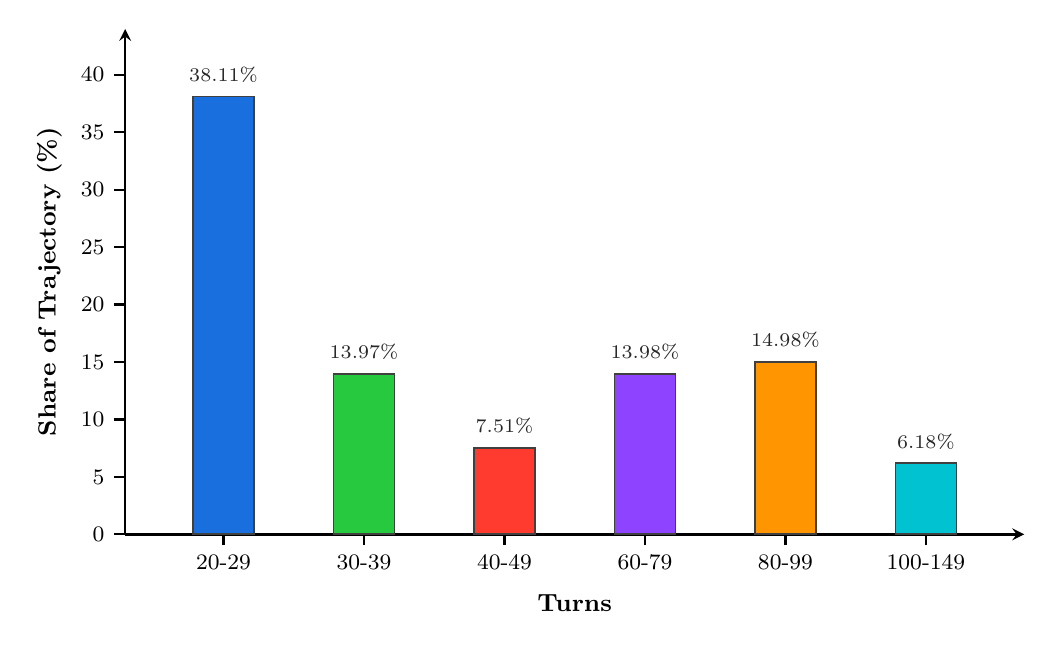
\begin{tikzpicture}
    \begin{axis}[
        width=13cm,
        height=8cm,
        xmin=0.3, xmax=6.7,
        ymin=0, ymax=44,
        ytick distance=5,
        ybar,
        bar width=22pt,
        axis lines=left,
        xlabel={Turns},
        ylabel={Share of Trajectory (\%)},
        xlabel style={font=\small\bfseries, yshift=-2pt},
        ylabel style={font=\small\bfseries},
        xtick={1,2,3,4,5,6},
        xticklabels={20-29, 30-39, 40-49, 60-79, 80-99, 100-149},
        xticklabel style={font=\footnotesize},
        yticklabel style={font=\footnotesize},
        tick align=outside,
        tick style={black, line width=0.8pt},
        major tick length=4pt,
        axis line style={black, line width=0.9pt},
        clip=false,
        % ---- 标签统一样式，不做数字格式化 ----
        nodes near coords style={
            font=\scriptsize, anchor=south, yshift=1.5pt, text=black!85,
        },
        bar shift=0pt,
        cycle list={},
    ]
    % ---- 每根柱子手动写标签文字，% 用 \% 转义 ----
    \addplot[ybar, fill=barA, draw=black!75, line width=0.6pt,
        nodes near coords={38.11\%}] coordinates {(1, 38.11)};
    \addplot[ybar, fill=barB, draw=black!75, line width=0.6pt,
        nodes near coords={13.97\%}] coordinates {(2, 13.97)};
    \addplot[ybar, fill=barC, draw=black!75, line width=0.6pt,
        nodes near coords={7.51\%}] coordinates {(3,  7.51)};
    \addplot[ybar, fill=barD, draw=black!75, line width=0.6pt,
        nodes near coords={13.98\%}] coordinates {(4, 13.98)};
    \addplot[ybar, fill=barE, draw=black!75, line width=0.6pt,
        nodes near coords={14.98\%}] coordinates {(5, 14.98)};
    \addplot[ybar, fill=barF, draw=black!75, line width=0.6pt,
        nodes near coords={6.18\%}] coordinates {(6,  6.18)};
    \end{axis}
\end{tikzpicture}

\end{document}
